%%%%%%%%%%%%%%%%%%%%%%%%%%%%%%%%%%%%%%%%%
%
% (c) 2018 by Jennifer Laaser
%
% This work is licensed under the Creative Commons Attribution-NonCommercial-ShareAlike 4.0 International License. To view a copy of this license, visit http://creativecommons.org/licenses/by-nc-sa/4.0/ or send a letter to Creative Commons, PO Box 1866, Mountain View, CA 94042, USA.
%
% The current source for these materials is accessible on Github: https://github.com/jlaaser/pogil-polymers
%
%%%%%%%%%%%%%%%%%%%%%%%%%%%%%%%%%%%%%%%%%

\renewcommand{\figpath}{content/polymchem/stepgrowth/dispersity/figs}

\begin{activity}[Molecular Weight Distributions in Step-Growth Polymerizations]

\begin{instructornotes}

	This activity introduces students to key concepts related to the molecular weight distributions obtained in step-growth polymerizations.
	
	After completing this activity, students will be able to:
			\begin{enumerate}
				\item ...
			\end{enumerate}
			
	\subsection*{Activity summary:}
	\begin{itemize}
		\item \textbf{Activity type:} Learning Cycle
		\item \textbf{Content goals:} Molecular weight distributions and dispersity in step-growth polymerizations
		\item \textbf{Process goals:} %https://pogil.org/uploads/attachments/cj54b5yts006cklx4hh758htf-process-skills-official-pogil-list-2015-original.pdf
			written communication, critical thinking, information processing
		\item \textbf{Duration:} TBD
		\item \textbf{Instructor preparation required:} none beyond knowledge of relevant content
		\item \textbf{Related textbook chapters:}
			\begin{itemize}
				\item \emph{Polymer Chemistry} (Hiemenz \& Lodge): section 2.4
			\end{itemize}
	\end{itemize}

\end{instructornotes}

	%\textbf{Focus question:} Put a central question for the students to consider through this exercise here.

\begin{model}[Probabilities of Forming Different Chain Lengths]

Suppose we perform a step-growth polymerization of AB-type monomers and stop the polymerization at extent of reaction $p$ (i.e. we stop the polymerization when the fraction of A groups that have reacted is equal to $p$).

Consider the following argument:
\begin{enumerate}
\item For a given AB-type monomer ($i=1$), 
\begin{itemize}
	\item the probability that the A group has \textit{not} reacted, and the monomer remains an AB monomer, is $1-p$.  This is the same as the probability of forming a chain with \emph{exactly} one monomer; while

	\item the probability that the A group \textit{has} reacted, and has formed at least an AbaB dimer, is $p$.
\end{itemize}

\item Of the dimers ($i=2$),
\begin{itemize}
	\item the probability that the A end group remains unreacted (and the chain stops growing) is $1-p$. Thus the probability of forming a dimer that remains a dimer, or a chain with exactly 2 monomers, is $(1-p)$ times the probability of forming a dimer in the first place ($p$), for a total probability of $(1-p)p$; while

	\item the probability that the A end group on the dimer reacts to form at least a trimer is $p$, so the total probability of forming at least a trimer is $p^2$.
\end{itemize}

\item Of the trimers ($i=3$),
\begin{itemize}
	\item the probability that the A end group remains unreacted (and the chain stops growing) is again $1-p$.  Thus the total probability of forming a chain with exactly three monomers is $(1-p)$ times the probability of forming a trimer in the first place ($p^2$), for a total probability of $(1-p)p^2$; while
	\item the probability that the A end group reacts to form at least a tetramer is $p$, for a total probability of $p^3$.
\end{itemize}

%We can represent this tree of probabilities graphically as follows:
\end{enumerate}

%\vspace{0.1in}
%\centerline{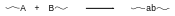
\includegraphics[width=0.6\textwidth]{\figpath/ABrxn.pdf}}

\end{model}

\vspace{0.05in}
\begin{ctqs}

	\question What is the probability of forming a chain with exactly four monomers ($i=4$)?
	
		\begin{solution}[0.6in]
			$(1-p)p^3$
		\end{solution}
	
	\question What is the probability of forming at least a pentamer ($i=5$)?
	
		\begin{solution}[0.6in]
			$p^4$
		\end{solution}
	
	\question Fill in the following table:
	
		\begin{center}
			\renewcommand{\arraystretch}{3.5}
			\begin{tabular}{|c|c|}
				\hline
				\textbf{~~i~~} & {\renewcommand{\arraystretch}{1}\begin{tabular}{c}\textbf{Probability of forming a chain of}\\\textbf{exactly $i$ monomers}\end{tabular} }\\\hline
				1 & \\\hline
				2 & \\\hline
				3 & \\\hline
				4 & \\\hline
				5 & \\\hline
			\end{tabular}
		\end{center}
	
	\question What pattern do you notice in these values?  Briefly describe your observations in 1-2 complete sentences.
	
		\begin{solution}[1.5in]
		\end{solution}
	
	\question Complete the following statement:
	
		``The probability of forming a chain with exactly $i$ monomers is \line(1,0){50}.''
	
		\begin{solution}[0.5in]
		\end{solution}
		
\end{ctqs}

\begin{infobox}

	The probability of making a chain of exactly length $i$ (i.e. the probability of making an $i$-mer that does not grow any longer) is the same as the %probability of given chain being an i-mer, because the number of chains of length $i$ is directly proportional to the probability of making a chain of length $i$.
	the mole fraction of chains with length $i$, which we also denote $x_i$.

\end{infobox}

\begin{ctqs}
	\question \label{stepdispersity:ctq:xi} What is the mole fraction of chains with length $i$?
	
		\begin{solution}[0.5in]
		\end{solution}
	
	\question Calculate the mole fractions of chains with length $i$ for $p=0.5$ and $p=0.9$, and use your results to fill in the following table:
	
		\begin{center}
			\renewcommand{\arraystretch}{4}
			\begin{tabular}{|c|c|c|}
				\hline
				\textbf{~~$i$~~} & $x_i$ when $p=0.5$ & $x_i$ when $p=0.9$ \\\hline
				1 & & \\\hline
				2 & & \\\hline
				3 & & \\\hline
				5 & & \\\hline
				10 & & \\\hline
				15 & & \\\hline
				20 & & \\\hline
			\end{tabular}
		\end{center}
		
		\clearpage
	\question Plot your results on the following axes.  Make sure to use a different symbol for points corresponding to $p=0.5$ than for the points corresponding to $p=0.9$.
	
		\begin{solution}[2.75in]
			\studentdisplay{
				\centerline{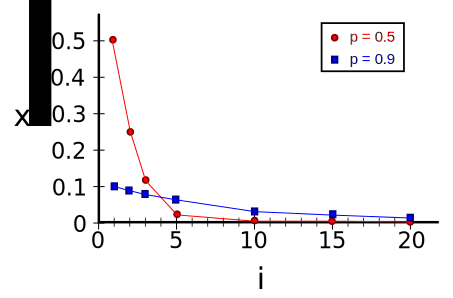
\includegraphics[width=0.7\textwidth]{\figpath/model1-xi-axes.pdf}}
			}
		\end{solution}
	
	\question How are the plots for $p=0.5$ and $p=0.9$ similar, and how are they different?  Briefly describe your observations in 2-3 complete sentences.
	
		\begin{solution}[1.5in]
		\end{solution}
	
	\question \label{stepdispersity:ctq:xiplus1} What is the mole fraction of chains with length $i+1$?
	
		\begin{solution}[0.5in]
		\end{solution}
	
	\question Compare your answer to question \ref{stepdispersity:ctq:xiplus1} with that to question \ref{stepdispersity:ctq:xi}. Can the mole fraction of chains with length $i+1$ ever be \emph{greater} than the mole fraction of chains with length $i$?  Justify your answer in 1-2 complete sentences.
	
		\begin{solution}[1.5in]
		\end{solution}
	
	\question Comment briefly on whether or not your answer to the preceding question is consistent with your plots.
	
		\begin{solution}[1in]
		\end{solution}
	
\end{ctqs}


\begin{model}[$M_n$ and $M_w$ for Step-Growth Polymerizations]

	To calculate $M_n$ and $M_w$, we need to know $n_i$, or the total number of chains with $i$ monomers.
	
	If we started with $v_A^0$ monomers, then when the extent of reaction is equal to $p$, there will be $(1-p)v_A^0$ unreacted A groups left.  Recalling that the number of unreacted A groups is equal to the number of molecules in the reaction mixture, this lets us write
	\begin{align*}
		n_i &= \text{(mole fraction of molecules that have length }i\text{) x (number of molecules in reaction mixture)}\\
			%&= (x_i)((1-p)v_A^0)\\
			&= \left(p^{i-1}(1-p)\right)\left((1-p)v_A^0\right)\\
			&= p^{i-1}(1-p)^2v_A^0
	\end{align*}
	
	If we plug this expression into our equation for $M_n$, we get
	\begin{equation*}
		M_n = \frac{\sum_i n_i M_i}{\sum_i n_i} %= \frac{\sum_i p^{i-1}(1-p)^2 v_A^0 i M_0}{\sum_i p^{i-1}(1-p)^2 v_A^0} 
		= M_0\frac{\sum_i p^{i-1}(1-p)^2 i }{\sum_i p^{i-1}(1-p)^2}
	\end{equation*}
	where $M_0$ is the molecular weight of the monomer ($M_i = M_0 i$).
	
	Evaluating these sums is a bit tedious, but if we do so, we obtain
	\begin{align*}
		M_n = \frac{M_0}{1-p} && \text{or} && N_n = \frac{M_n}{M_0} = \frac{1}{1-p}
	\end{align*}
	which is exactly what we expected (whew - our math worked!).
	
	Similarly, if we plug this expression into our equation for $M_w$ and work through the sums, we get
	\begin{align*}
		M_w = \frac{\sum_i n_i M_i^2}{\sum_i n_i M_i} = M_0\frac{1+p}{1-p} && \text{or} && N_w = \frac{M_w}{M_0} = \frac{1+p}{1-p}
	\end{align*}

\end{model}

\begin{ctqs}
		\question Calculate the dispersity for a step-growth reaction with extent of reaction $p$.
		
			\begin{solution}[1in]
			\end{solution}
			
			
		\question What is the value of the dispersity when $p=0$?  Briefly comment on whether or not this answer makes sense.
		
			\begin{solution}[1.5in]
			\end{solution}
			
			
		\question What is the value of the dispersity when $p=1$?
		
			\begin{solution}[0.5in]
			\end{solution}
			
			
			
		\question Can the dispersity of a polymer produced by step-growth polymerization ever be greater than 2?  Briefly defend your answer in 1-2 complete sentences.
		
			\begin{solution}[1in]
			\end{solution}
			
			
\end{ctqs}

\begin{exercises}

		\exercise Suppose you synthesized a polymer by step-growth polymerization and found that it had a dispersity of 1.86.
		
			\begin{enumerate}
				\item What must the extent of reaction have been in this polymerization?
		
					\begin{solution}%[1in]
					\end{solution}
					
				\item What would you expect the number-average degree of polymerization of this polymer to be?
		
					\begin{solution}%[1in]
					\end{solution}
			\end{enumerate}
\end{exercises}
	
\end{activity}